\documentclass{article}

\usepackage{graphicx}
\usepackage{tikz}
\usepackage{tikzsymbols}
\usetikzlibrary{calc,patterns,shapes.geometric}
\pagestyle{empty}
\usepackage[margin=0pt]{geometry}
\geometry{papersize={14in,12in}}

\def\centerarc[#1](#2)(#3:#4:#5){\draw[#1] ($(#2)+({#5*cos(#3)},{#5*sin(#3)})$) arc (#3:#4:#5);}

\begin{document}
	\begin{figure}
		\centering
		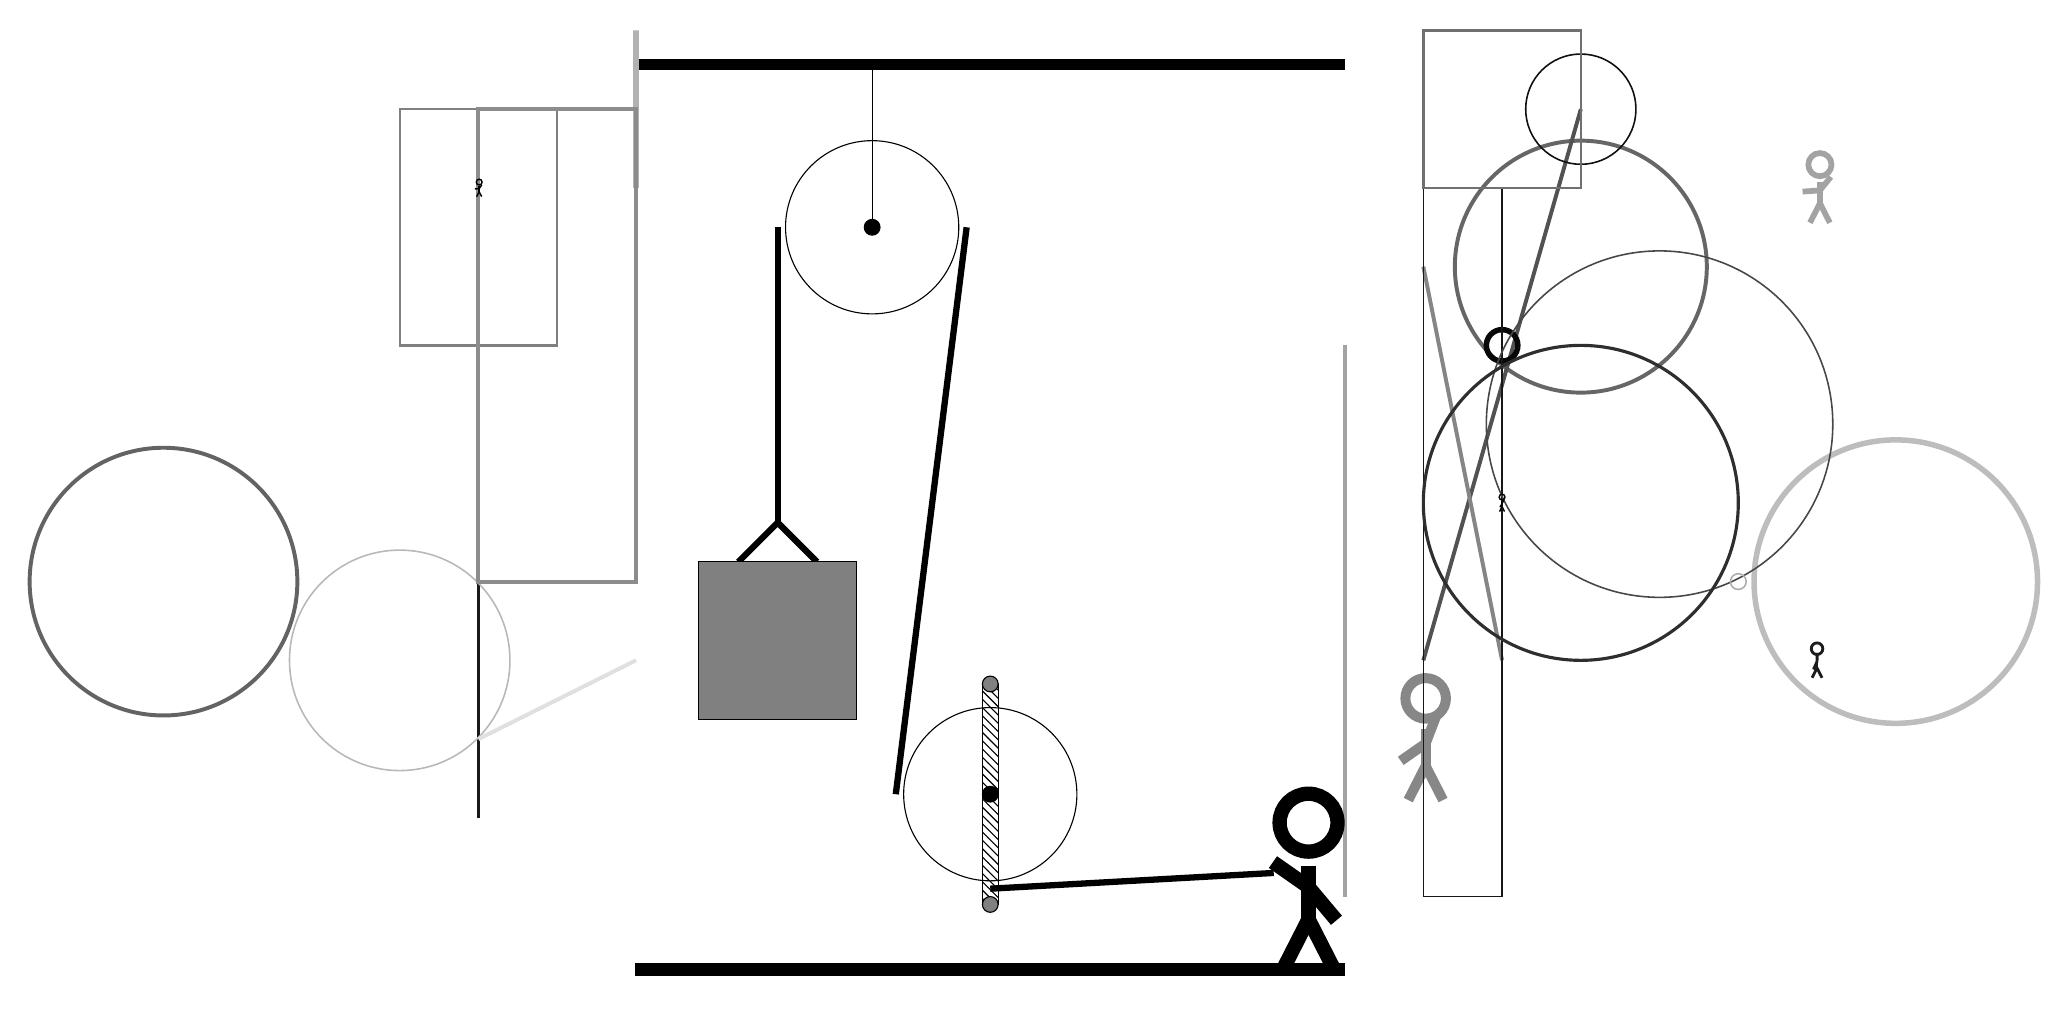
\begin{tikzpicture}
			%%%%% START %%%%%
			
			\draw[fill=black] (-2, 11.5) rectangle (7, 11.625);
			
			\draw (1, 9.5) circle (1.1);
			\draw[fill=black] (1, 9.5) circle (0.1);
			\draw (1, 11.5) -- (1, 9.5);
			
			\draw[fill=white](2.5, 2.3) circle (1.1);
			\draw[fill=black] (2.5, 2.3) circle (0.1);
			\draw[pattern=north west lines, pattern color=black] (2.4, 3.7) rectangle (2.6, 0.9);
			\draw[fill=black!50] (2.5, 3.7) circle (0.1);
			\draw[fill=black!50] (2.5, 0.9) circle (0.1);
			
			\draw[line width=0.8mm] (-0.7, 5.25) -- (-0.2, 5.75) -- (0.3, 5.25);
			\draw[fill=black!50] (-1.2, 5.25) rectangle (0.8, 3.25);
			
			\node[line width=0.7mm, color=black!47] at (8, 3) {\Strichmaxerl[7][35][69]};
			
			\draw[line width=0.5mm, color=black!36](7, 1) -- (7, 8);
			\draw [line width=0.5mm, color=black!60](10, 9) circle (1.6);
			\draw [line width=0.7mm, color=black!26](14, 5) circle (1.8);
			\draw[line width=0.3mm, color=black!90] (-4, 11) rectangle (-4, 2);
			
			\draw[line width=0.5mm, color=black!68](8, 4) -- (10, 11);
			\draw[line width=0.3mm, color=black!50] (-3, 8) rectangle (-5, 11);
			\draw [line width=0.7mm, color=black!97](9, 8) circle (0.2);
			\draw[line width=0.5mm, color=black!48](8, 9) -- (9, 4);
			\draw [line width=0.2mm, color=black!28](-5, 4) circle (1.4);
			\draw[line width=0.7mm, color=black!30] (-2, 10) rectangle (-2, 12);
			\draw[line width=0.2mm, color=black!91] (8, 10) rectangle (9, 1);
			\draw [line width=0.2mm, color=black!94](10, 11) circle (0.7);
			
			\draw [line width=0.2mm, color=black!72](11, 7) circle (2.2);
			\draw[line width=0.3mm, color=black!56] (8, 12) rectangle (10, 10);
			\draw [line width=0.2mm, color=black!32](12, 5) circle (0.1);
			
			\node[line width=0.4mm, color=black!89] at (13, 4) {\Strichmaxerl[2][66][89]};
			
			\draw[line width=0.5mm, color=black!45] (-4, 11) rectangle (-2, 5);
			\node[line width=0.3mm, color=black!97] at (9, 6) {\Strichmaxerl[1][60][62]};
			\node[line width=0.2mm, color=black!36] at (13, 10) {\Strichmaxerl[4][4][51]};
			\node[line width=0.2mm, color=black!100] at (-4, 10) {\Strichmaxerl[1][6][54]};
			
			\draw [line width=0.4mm, color=black!82](10, 6) circle (2.0);
			\draw[line width=0.5mm, color=black!12](-4, 3) -- (-2, 4);
			\draw [line width=0.5mm, color=black!61](-8, 5) circle (1.7);
			
			\draw[line width=0.8mm] (-0.2, 9.5) -- (-0.2, 5.75);
			\centerarc[line width=0.8mm](1, 9.5)(0:180:1.2000000000000002);
			\draw[line width=0.8mm](2.2, 9.5) -- (1.3, 2.3);
			\centerarc[line width=0.8mm](2.5, 2.3)(180:270:1.2000000000000002);
			\draw[line width=0.8mm](2.5, 1.1) -- (6.1, 1.3);
			
			\node at (6.5, 1.2) {\Strichmaxerl[10][-35][-50]};
			
			\draw[fill=black] (-2, 0) rectangle (7, 0.15);
			
			%%%%% END %%%%%
		\end{tikzpicture}
	\end{figure}	
\end{document}